% Week 06 slides: conda environments and the working directory.
%
% Compile with XeLaTeX, not pdfLaTeX: the fonts are loaded with fontspec.
%
% In Positron, LaTeX Workshop's build button uses the "latexmk (XeLaTeX)" recipe
% in .vscode/settings.json. From a terminal, the same command is:
%
%     latexmk -xelatex -auxdir=.latex-build -outdir=. 06-conda.tex
%
% Auxiliary files go in .latex-build/, which is gitignored. Only this file and
% 06-conda.pdf are committed.

\documentclass[aspectratio=169,11pt]{beamer}

\usetheme[progressbar=frametitle, numbering=fraction]{metropolis}
\usepackage{amssymb}
\usepackage{pifont}

% Load Fira Mono by file name: XeLaTeX on Windows does not always find it by
% its font name, and falls back to a slanted substitute.
\setmonofont{FiraMono}[Extension=.otf, UprightFont=*-Regular, BoldFont=*-Bold, Scale=0.92]
\usepackage{tikz}
\usetikzlibrary{arrows.meta, positioning, fit}

% ---------------------------------------------------------------------------
% Colors: the course palette, taken from the "Your turn" box in the notebooks
% ---------------------------------------------------------------------------
\definecolor{ban}{HTML}{31708F}
\definecolor{banlight}{HTML}{D9EDF7}
\definecolor{good}{HTML}{3C763D}
\definecolor{bad}{HTML}{A94442}
\definecolor{softgray}{HTML}{6C757D}

\setbeamercolor{frametitle}{bg=ban, fg=white}
\setbeamercolor{progress bar}{fg=banlight, bg=ban!60}
\setbeamercolor{title separator}{fg=ban}
\setbeamercolor{alerted text}{fg=bad}
\setbeamercolor{block title}{bg=banlight, fg=ban}
\setbeamercolor{block body}{bg=banlight!40}

% Inline code and a highlighted keyword
\newcommand{\code}[1]{\texttt{#1}}
\newcommand{\key}[1]{\textbf{\textcolor{ban}{#1}}}
\newcommand{\ui}[1]{\textbf{#1}}

% The label above an exercise slide's title
\newcommand{\exerciseframe}[3]{%
  \begin{frame}[t]{#1}
    \vspace{0.4em}
    {\small\textcolor{softgray}{\textsc{exercise}}}\par\vspace{0.6em}
    #2
    \vfill
    \begin{block}{Steps}
      All steps and checks are in \key{exercises.md}. #3
    \end{block}
    \vspace{0.6em}
  \end{frame}}

\title{Environments and the working directory}
\subtitle{Week 06 workshop}
\author{BAN405 Python Programming for Data Science}
\date{}

\begin{document}

\maketitle

% ===========================================================================
\section{Why}
% ===========================================================================

\begin{frame}{Last week: your work cannot be lost}
  \begin{itemize}
    \item Your BAN405 folder is a repository, and it is on GitHub.
    \item Every commit is a snapshot you can go back to.
  \end{itemize}
  \vspace{1em}
  \begin{block}{Today's question}
    A classmate clones your repository tonight and runs your notebooks.\\[0.3em]
    \textbf{Do they run?}
  \end{block}
  \vspace{0.8em}
  Not necessarily. git keeps your code, but your code is not the whole program.
\end{frame}

\begin{frame}{Two lines, and what they depend on}
  Almost every notebook in the rest of the course starts like this:
  \vspace{0.8em}

  \centering
  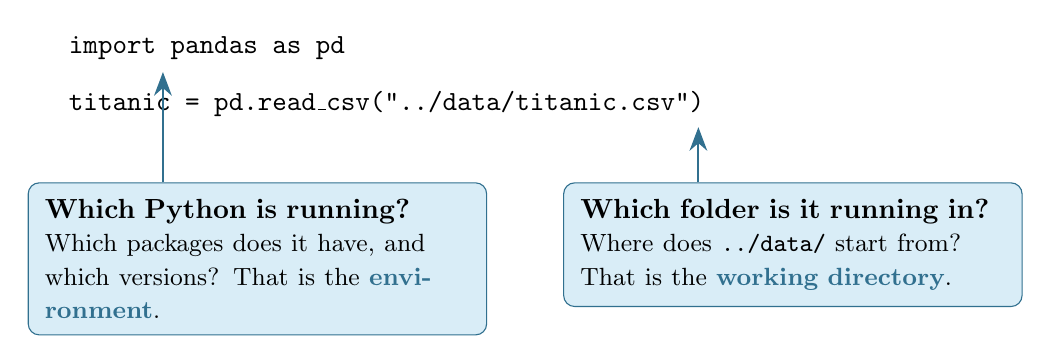
\begin{tikzpicture}[
      note/.style={draw=ban, fill=banlight, rounded corners, text width=5.4cm, align=left,
                   inner sep=6pt},
      arr/.style={-{Stealth[length=3mm]}, thick, ban}]
    \node[anchor=west, font=\ttfamily] (l1) at (0, 0) {import pandas as pd};
    \node[anchor=west, font=\ttfamily] (l2) at (0, -0.7) {titanic = pd.read\_csv("../data/titanic.csv")};
    \node[note, anchor=north west] (env) at (-0.4, -1.7)
      {\textbf{Which Python is running?}\\\small Which packages does it have, and which versions? That is the \key{environment}.};
    \node[note, anchor=north west] (wd) at (6.4, -1.7)
      {\textbf{Which folder is it running in?}\\\small Where does \code{../data/} start from? That is the \key{working directory}.};
    \draw[arr] (env.north) ++(-1.2, 0) -- ++(0, 1.4);
    \draw[arr] (wd.north) ++(-1.2, 0) -- ++(0, 0.7);
  \end{tikzpicture}

  \vspace{1em}
  \raggedright
  Neither is written in your code. Today you learn to see both, and to control both.
\end{frame}

\begin{frame}{Today}
  Six exercises. Each builds on the one before.
  \vspace{0.8em}

  \centering
  \begin{tabular}{c l l}
    & \textbf{What you do} & \textbf{Where} \\ \hline
    1 & Create an environment and use it & terminal, Positron \\
    2 & Write it to a file, delete it, rebuild it & terminal \\
    3 & Build the course environment & terminal, Positron \\
    4 & Read a data file from a notebook & Positron \\
    5 & Run someone else's project & Positron, terminal \\
    6 & Make your own repository runnable & Positron, GitHub \\
  \end{tabular}

  \vspace{1em}
  \raggedright
  Explanations, options and fixes are in the \key{conda guide}, in the \code{guides} folder.
\end{frame}

% ===========================================================================
\section{Environments}
% ===========================================================================

\begin{frame}{``Python'' is not one thing on your laptop}
  \begin{columns}[T]
    \begin{column}{0.5\textwidth}
      What \code{import pandas} gives:
      \begin{itemize}
        \item \code{ModuleNotFoundError}
        \item an older pandas, from an earlier course
        \item a newer pandas, installed for something else
        \item a Python that is not even Miniforge's
      \end{itemize}
    \end{column}
    \begin{column}{0.46\textwidth}
      \begin{itemize}
        \item Packages change between versions. Code that works with one can fail, or quietly give another answer, with the next.
        \item Upgrade pandas for this course, and a project from an earlier one may stop working.
      \end{itemize}
    \end{column}
  \end{columns}
  \vspace{1.2em}
  \centering
  The course material is written for \emph{one} set of versions. How do we all get it,\\
  without breaking whatever you already have?
\end{frame}

\begin{frame}{An environment}
  \begin{columns}[T]
    \begin{column}{0.5\textwidth}
      \begin{itemize}
        \item A \key{folder} with its own copy of Python and its own packages.
        \item One per project. Installing into one cannot change another.
        \item You switch with \code{conda activate}. The prompt shows where you are: \code{(base)}, \code{(practice)}.
      \end{itemize}
    \end{column}
    \begin{column}{0.46\textwidth}
      \ttfamily\small
      \textcolor{softgray}{miniforge3/}\\
      ├── python \ \ \ \ \ \ \ \textcolor{ban}{$\leftarrow$ base}\\
      └── envs/\\
      \ \ \ \ ├── practice/\\
      \ \ \ \ ├── ban405/\\
      \ \ \ \ └── temperature-app/
    \end{column}
  \end{columns}
  \vspace{1em}
  \begin{block}{\code{base}}
    The environment conda uses for itself. Whatever is in it already, leave it, and do not add to it.
  \end{block}
\end{frame}

\begin{frame}{Where packages come from: conda-forge}
  \begin{itemize}
    \item \key{conda} downloads packages, and works out which versions fit together.
    \item It downloads them from a \key{channel}. Ours is \key{conda-forge}: a large collection, maintained by volunteers.
    \item \code{conda-forge.org/packages}: every package, and every version of it.
  \end{itemize}
  \vspace{0.6em}
  \begin{block}{Together: before you start}
    Mac: \textbf{Terminal}. Windows: \textbf{Miniforge Prompt}.\\[0.3em]
    \code{conda --version}\\
    \code{conda env list} \\
    \code{conda config --show channels}\\[0.3em]
  \end{block}
\end{frame}

\exerciseframe{Exercise 1 --- Create an environment and use it}{%
  \begin{itemize}
    \item \textbf{Together, in the terminal:} create \code{practice}, with Python 3.14 and pandas. Compare it with \code{base}.
    \item \textbf{On your own, in Positron:} a notebook that prints which Python runs it, and which pandas.
    \item Run the same cell with \code{practice}, then with \code{base}.
  \end{itemize}}{Mac: \textbf{Terminal}. Windows: \textbf{Miniforge Prompt}.}

\begin{frame}{What you just saw}
  \begin{itemize}
    \item The \key{terminal} is where environments are made.
    \item \key{Positron} is where you choose which one runs your code: the \ui{kernel selector}.
    \item \code{sys.executable} tells you which Python is running. Its path ends in \code{envs/practice}.
  \end{itemize}
  \vspace{0.8em}
  \begin{block}{The lesson}
    Same code, same computer, different result. It depends on which environment runs it.\\[0.3em]
    \code{ModuleNotFoundError} for a package you know you installed? Wrong environment.
  \end{block}
\end{frame}

\begin{frame}{An environment as a file}
  \begin{columns}[T]
    \begin{column}{0.44\textwidth}
      \ttfamily\small
      name: practice\\
      channels:\\
      \ \ - conda-forge\\
      dependencies:\\
      \ \ - pandas\\
      \ \ - python=3.14\\
      \textcolor{softgray}{prefix: ...}
    \end{column}
    \begin{column}{0.52\textwidth}
      \code{conda env export --from-history}\\
      \code{\ \ \ \ > practice.yml}
      \vspace{0.6em}
      \begin{itemize}
        \item The packages \emph{you asked for}, and where they come from.
        \item Anyone can rebuild it:\\\code{conda env create --file practice.yml}
      \end{itemize}
    \end{column}
  \end{columns}
  \vspace{1em}
  \centering
  The file is the recipe. The environment itself is disposable.
\end{frame}

\exerciseframe{Exercise 2 --- Write it down, delete it, rebuild it}{%
  \begin{itemize}
    \item \textbf{Together:} go to your \code{week06} folder with \code{cd}. Copy the path, do not type it.
    \item \textbf{On your own:} export \code{practice} to \code{practice.yml}, and delete the environment.
    \item Open a \emph{new} terminal, and rebuild it from the file.
  \end{itemize}}{One step fails on purpose. Read the error.}

\begin{frame}{What went wrong, and why}
  \begin{itemize}
    \item A terminal is always \emph{in} a folder: its \key{working directory}. A new one starts in your home folder.
    \item \code{--file practice.yml} means \emph{``\code{practice.yml}, in the folder I am in''}.
    \item The error names the exact path conda tried. The file was fine. The command ran in the wrong place.
  \end{itemize}
  \vspace{0.8em}
  \begin{block}{Where am I?}
    \textbf{Windows:} the prompt shows it: \code{(base) C:\textbackslash Users\textbackslash you\textbackslash BAN405\textbackslash week06>}\\
    \textbf{Mac:} the prompt shows the folder's name; \code{pwd} prints the whole path.
  \end{block}
  \vspace{0.4em}
  Keep this error in mind. You meet it again in a notebook, where no prompt tells you where you are.
\end{frame}

\begin{frame}{Pinned versions}
  \begin{columns}[T]
    \begin{column}{0.5\textwidth}
      \code{python=3.14 pandas}
      \begin{itemize}
        \item ``The newest that fits, today.''
        \item Build it next month, get something else.
      \end{itemize}
      \vspace{0.6em}
      \code{pandas=3.0.3}
      \begin{itemize}
        \item ``Exactly this one, always.''
        \item Every laptop, every month, the same.
      \end{itemize}
    \end{column}
    \begin{column}{0.46\textwidth}
      \textbf{The course environment}\\[0.3em]
      \ttfamily\footnotesize
      name: ban405\\
      channels:\\
      \ \ - conda-forge\\
      \ \ - nodefaults\\
      dependencies:\\
      \ \ - python=3.14.6\\
      \ \ - numpy=2.5.1\\
      \ \ - pandas=3.0.3\\
      \ \ - matplotlib=3.11.0\\
      \ \ - statsmodels=0.14.6\\
      \ \ \textcolor{softgray}{...}
    \end{column}
  \end{columns}
  \vspace{0.8em}
  Version pinning ensures that you (and everyone else) gets the exact same version of a package every time.
\end{frame}

\exerciseframe{Exercise 3 --- Build the course environment}{%
  \begin{itemize}
    \item Build \code{ban405} straight from its web address: no download first.
    \item Switch \code{checks.ipynb} to the \code{ban405} kernel, and run it again.
    \item Compare its pandas with the one \code{practice} got.
  \end{itemize}}{It takes a few minutes: read the file while it runs.}

% ===========================================================================
\section{The working directory}
% ===========================================================================

\begin{frame}{Every running program is somewhere}
  A \key{relative path} like \code{data/titanic.csv} is read starting from the \key{working directory}.
  \vspace{0.8em}

  \centering
  \begin{tabular}{l l}
    \textbf{Running in} & \textbf{Working directory} \\ \hline
    a terminal & where you \code{cd}'d to: the prompt shows it \\
    a notebook & \key{the folder the notebook is saved in} \\
    a script, with ▶ in Positron & the folder open in Positron \\
  \end{tabular}

  \vspace{1em}
  \raggedright
  \begin{itemize}
    \item \code{os.getcwd()} prints it from inside Python.
    \item \code{..} means \emph{the folder above}.
  \end{itemize}
\end{frame}

\exerciseframe{Exercise 4 --- Where your notebook looks for files}{%
  \begin{itemize}
    \item \textbf{Part A:} in \code{week06/checks.ipynb}, find the working directory, and read \code{titanic.csv} until it works.
    \item \textbf{Part B:} the same line, in a notebook at the top of your BAN405 folder.
    \item pandas and matplotlib today are a demonstration. They are the rest of the course.
  \end{itemize}}{}

\begin{frame}{Why the course writes \code{../data/}}
  \begin{columns}[T]
    \begin{column}{0.48\textwidth}
      \ttfamily\small
      BAN405/\\
      ├── data/\\
      │\ \ \ └── titanic.csv\\
      └── week06/\\
      \ \ \ \ └── checks.ipynb \textcolor{ban}{$\leftarrow$ here}\\[0.6em]
      \normalfont\normalsize
      \code{"../data/titanic.csv"}\\
      {\small up one folder, into \code{data}}
    \end{column}
    \begin{column}{0.48\textwidth}
      \ttfamily\small
      project/\\
      ├── data/\\
      │\ \ \ └── titanic.csv\\
      └── analysis.ipynb \textcolor{ban}{$\leftarrow$ here}\\[2.05em]
      \normalfont\normalsize
      \code{"data/titanic.csv"}\\
      {\small straight into \code{data}}
    \end{column}
  \end{columns}
  \vspace{1em}
  \begin{block}{The rule}
    A path in a notebook is written \textbf{from the folder the notebook is saved in}. Know where the notebook is and where the data is, and you can always write it.
  \end{block}
\end{frame}

\begin{frame}{Four ways to point at a file}
  \centering
  \begin{tabular}{l l l}
    & \textbf{Example} & \textbf{Works} \\ \hline
    Relative & \code{"../data/titanic.csv"} & wherever the project goes \\
    Relative & \code{"data/titanic.csv"} & the same, for a notebook at the top \\
    Absolute & \code{r"C:\textbackslash Users\textbackslash you\textbackslash ..."} & \alert{only on your own computer} \\
    Web address & \code{"https://..."} & anywhere, \alert{but only online} \\
  \end{tabular}

  \vspace{1.2em}
  \raggedright
  The course uses relative paths. A project keeps working when it moves, as long as the notebook and the data keep their places relative to each other.\\[0.4em]
  {\small The other two are an optional exercise at home.}
\end{frame}

\begin{frame}[t]{Demo: a script is not a notebook}
  \vspace{0.3em}
  {\small\textcolor{softgray}{\textsc{live demo}}}\par\vspace{0.4em}
  \begin{enumerate}
    \item In \code{week06}, a script \code{read\_titanic.py} with the line that worked in the notebook:\\
      \code{pd.read\_csv("../data/titanic.csv")}
    \item Run it with ▶. \code{FileNotFoundError}.
    \item \code{print(os.getcwd())}: the BAN405 folder, not \code{week06}.
  \end{enumerate}
  \vfill
  \begin{block}{Why}
    A script run with ▶ runs from the folder open in Positron, not from its own folder. The rest of the course is notebooks, so you will rarely meet this. But when you do, you know why.
  \end{block}
\end{frame}

% ===========================================================================
\section{Projects}
% ===========================================================================

\exerciseframe{Exercise 5 --- Run someone else's project}{%
  \begin{itemize}
    \item Clone \code{temperature-app} into \code{git-practice}: your converter, as a web app.
    \item Try it in \code{ban405} first. Then follow its README.
    \item Convert 212\,°F in your browser.
  \end{itemize}}{The app keeps running until you press \code{Ctrl+C} in the terminal.}

\begin{frame}{What makes a project runnable}
  \begin{columns}[T]
    \begin{column}{0.5\textwidth}
      \ttfamily\footnotesize
      temperature-app/\\
      ├── .gitignore\\
      ├── README.md \ \ \ \ \ \ \ \ \textcolor{ban}{$\leftarrow$ how to run}\\
      ├── app.py\\
      ├── environment.yml \ \textcolor{ban}{$\leftarrow$ what it needs}\\
      └── temperature\_tools.py
    \end{column}
    \begin{column}{0.46\textwidth}
      \begin{enumerate}
        \item \textbf{The code}, in a repository.
        \item \textbf{The data}, read with relative paths.
        \item \textbf{An environment file}, with the versions that matter pinned.
        \item \textbf{A README} that says how to run it.
      \end{enumerate}
    \end{column}
  \end{columns}
  \vspace{1.2em}
  \centering
  You ran a project you had never seen, with a package you had never used,\\
  without installing anything by hand.
\end{frame}

\exerciseframe{Exercise 6 --- Make your own repository runnable}{%
  \begin{itemize}
    \item Add the course's \code{environment.yml} to the top of your BAN405 folder.
    \item Add a \emph{How to run} section to your README.
    \item Commit, and push. Look at the result on GitHub.
  \end{itemize}}{}

% ===========================================================================
\section{From now on}
% ===========================================================================

\begin{frame}{conda and pip}
  \begin{itemize}
    \item \key{pip} is Python's own installer, and it works inside a conda environment too.
    \item \textbf{Prefer conda.} It checks that all your packages fit together before installing anything.
    \item \textbf{Use pip when conda cannot help}: a package that is not on conda-forge.
    \item \textbf{conda first, then pip.} Installing with conda afterwards can undo what pip did.
  \end{itemize}
  \vspace{0.8em}
  \begin{block}{Careful}
    \code{--from-history} does not record what pip installed. Add those packages to the file by hand.
  \end{block}
\end{frame}

\begin{frame}{Habits}
  \begin{columns}[T]
    \begin{column}{0.48\textwidth}
      \textbf{Environments}
      \begin{itemize}
        \item One environment per project.
        \item Leave \code{base} alone.
        \item Pin the versions that matter.
        \item Keep \code{environment.yml} next to the code.
        \item Delete environments you no longer use.
      \end{itemize}
    \end{column}
    \begin{column}{0.48\textwidth}
      \textbf{Every session from now on}
      \begin{enumerate}
        \item Open your \textbf{BAN405 folder} in Positron.
        \item Choose the \key{ban405} kernel.
        \item Read data with \code{../data/}.
        \item Commit as you work. Push when you finish.
      \end{enumerate}
    \end{column}
  \end{columns}
\end{frame}

\begin{frame}[t]{What you did today}
  \begin{columns}[T]
    \begin{column}{0.52\textwidth}
      \textbf{Today you}
      \footnotesize
      \begin{itemize}
        \item created, deleted and rebuilt an environment
        \item built the course environment from a file
        \item found out where a notebook looks for files
        \item ran someone else's project from its README
        \item made your own repository runnable
      \end{itemize}
    \end{column}
    \begin{column}{0.44\textwidth}
      \textbf{At home} {\small (in \key{exercises.md})}
      \footnotesize
      \begin{itemize}
        \item Finish Exercise 6, if needed.
        \item Delete \code{practice} and \code{temperature-app}. \textbf{Keep \code{ban405}}.
        \item \emph{Optional:} absolute paths and web addresses; test your repository from a fresh clone.
      \end{itemize}
    \end{column}
  \end{columns}
  \vfill
  \begin{block}{Next week}
    Data. Reading a file into a table with pandas, and getting it into a shape you can trust.
  \end{block}
\end{frame}

\end{document}
